\documentclass[
      12pt,
            Review ]{article}






% --- type and typeface? -----------------------

% input
\usepackage[utf8]{inputenc}

% typography
\usepackage{microtype}


\usepackage[T1]{fontenc}


% text block
\usepackage{setspace}
\usepackage[              margin = 1in 
                        ]{geometry}

\usepackage{enumitem}
  \setlist{noitemsep}



% decimal numbering for appendix figs and tabs


% Deletes section counters
% \setcounter{secnumdepth}{0}







  \usepackage{longtable, booktabs}

  \usepackage{graphicx,grffile}
  % Scale images; don't overflow page margins by default.
  % Still possible explicate \includegraphics[width, height, ...]{}
  \makeatletter
    \def\maxwidth{\ifdim\Gin@nat@width>\linewidth\linewidth\else\Gin@nat@width\fi}
    \def\maxheight{\ifdim\Gin@nat@height>\textheight\textheight\else\Gin@nat@height\fi}
  \makeatother 
  \setkeys{Gin}{width=\maxwidth,height=\maxheight,keepaspectratio}








  \usepackage{natbib}
  \bibliographystyle{apa}
  % protect underscores in most circumstances
  \usepackage[strings]{underscore} 


% 

% \newtheorem{hypothesis}{Hypothesis}

\makeatletter
  \@ifpackageloaded{hyperref}{}{%
    \ifxetex
      % page size defined by xetex
      % unicode breaks when used with xetex
      \PassOptionsToPackage{hyphens}{url}\usepackage[setpagesize = false, 
                                                     unicode = false, 
                                                     xetex]{hyperref}
    \else
      \PassOptionsToPackage{hyphens}{url}\usepackage[unicode = true]{hyperref}
    \fi
  }

  \@ifpackageloaded{color}{
    \PassOptionsToPackage{usenames,dvipsnames}{color}
  }{
    \usepackage[usenames,dvipsnames]{color}
  }
\makeatother

\hypersetup{breaklinks = true,
            bookmarks = true,
            pdfauthor = {Devin Judge-Lord (University of Wisconsin--Madison) and Constance L. McDermott (Oxford University) and Benjamin Cashore (Yale University)},
             pdfkeywords  =  {policy change, private authority, certification, corporate social
responsibility, private governance},  
            pdftitle = {Do Private Regulations Ratchet Up?: How to distinguish types of regulatory stringency and patterns of change},
            colorlinks = true,
            citecolor = black,
            urlcolor = blue,
            linkcolor = magenta,
            pdfborder = {0 0 0}}

% \urlstyle{same}  % don't use monospace font for urls


% set default figure placement to htbp
\makeatletter
  \def\fps@figure{hbtp}
\makeatother


% optional footnotes as endnotes
  \usepackage{endnotes}
  \renewcommand{\enotesize}{\normalsize}
  \let\footnote = \endnote


% ----- Pandoc wants this tightlist command ----------
\providecommand{\tightlist}{
  \setlength{\itemsep}{0pt}
  \setlength{\parskip}{0pt}
}





% --- title & section styles -----------------------


% title, author, date
  \title{Do Private Regulations Ratchet Up?: 
           \\ How to distinguish types of regulatory stringency and patterns of change\thanks{We are grateful to reviewers of earlier versions of this paper presented
to the American Politics Workshop at the University of
Wisconsin-Madison, the Association of Public Policy Analysis and
Management (APPAM) Annual Research Conference, and the Association of
Environmental Studies and Sciences Annual Meeting. We are also grateful
to extensive feedback on a 2014 draft of the analytic framework and the
underlying data tables from officials from the Forest Stewardship
Council (FSC), the Sustainable Forestry Initiative (SFI), and the
Program for the Endorsement of Forest Certification (PEFC). We are
grateful for funding from the Fox Foundation, Procter \& Gamble,
Staples, Office Depot, and Arup. We also thank Erica Pohnan and Akiva
Fishman for research and editing assistance. The authors are fully
responsible for data collection, analysis, and any errors. Comments
welcome:
\href{mailto:JudgeLord@Wisc.edu}{\nolinkurl{JudgeLord@Wisc.edu}}. The
most version of this paper is available at
\url{https://judgelord.github.io/FSC-SFI/oe/certification.pdf}.}}

  \author{ % author, option footnote, optional affiliation
            Devin Judge-Lord  \\ \emph{University of Wisconsin--Madison} 
             \and 
           % author, option footnote, optional affiliation
            Constance L. McDermott  \\ \emph{Oxford University} 
             \and 
           % author, option footnote, optional affiliation
            Benjamin Cashore  \\ \emph{Yale University} 
            }

% auto-format date?
  \date{May 15, 2019}


% abstract
\usepackage{abstract}
  \renewcommand{\abstractname}{}    % clear the title
  \renewcommand{\absnamepos}{empty} % originally center

  \newcommand*{\authorfont}{\sffamily\selectfont}


% section titles
\usepackage[small, bf, sc]{titlesec}
  % \titleformat*{\subsection}{\itshape}
  \titleformat*{\subsubsection}{\itshape} 
  \titleformat*{\paragraph}{\itshape} 
  \titleformat*{\subparagraph}{\itshape}




\usepackage{floatrow}
\floatsetup[figure]{capposition=top}
\floatsetup[table]{capposition=top}
\usepackage{multirow}
\usepackage{rotating} 
\usepackage{caption}




\begin{document}
 

% --- PAGE: title and abstract -----------------------

  \maketitle

% \pagenumbering{gobble}



  \begin{abstract}
    \noindent Due to inconsistent measures of regulatory stringency, scholars offer
conflicting accounts about whether competing private governance
initiatives ``race to the bottom,'' ``ratchet up,'' ``converge,'' or
``diverge.'' To remedy this, we offer a framework to distinguish three
often-conflated measures: regulatory scope, prescriptiveness, and
performance levels. We use our framework to compare competing U.S.
forestry certification programs, one founded by environmental activists
and their allies, the other by the American Forest \& Paper Association.
We find ``upward'' but also divergent policy prescriptiveness, with the
activist-founded program adding requirements that impose costs on firms
and the industry-backed program mostly adding requirements with net
benefits to the sector. These results are consistent with the hypothesis
that industry-backed programs emphasize less costly types of stringency
than activist-backed programs. Furthermore, we find several more nuanced
patterns of change that previous scholarship failed to anticipate,
illustrating how disentangling types of stringency can improve theory
building and testing. 

          \hfill \\ 
      \noindent \emph{Keywords}: policy change, private authority, certification, corporate social
responsibility, private governance 
    
  \end{abstract}



% --- PAGE: contents -----------------------




% --- PAGE: body -----------------------



\noindent 
      \doublespacing 
    \newpage

\section{Introduction}\label{introduction}

Private governance initiatives, such as product certification programs,
have targeted farm and factory working conditions, greenhouse gas
emissions, and fishery, mine, and forest management
\citep{Auld2014, Bartley2003, Bozzi2012, Hudson2003, VanderVen2015, Vince2017}.
Many of these programs were founded by activists who were dissatisfied
with public regulations. Using tactics such as boycotts as ``sticks''
and brand-boosting praise as ``carrots,'' activists attempt to pressure
companies to comply with certification programs that go beyond the
requirements of public laws \citep{Cashore2002}. When buyers add
certification criteria to their purchasing policies and contracts, those
certification programs gain power to regulate how commodities are
produced. Industry groups often resist these efforts at private
(i.e.~non-state) regulation, in some cases launching competing
certification programs to offer more ``business-friendly'' alternatives.

Debates among supporters of activist-backed programs and industry-backed
alternatives often center on the relative stringency of each program's
regulatory requirements. Compared to governments, which enjoy sovereign
authority, it is especially vital for private organizations to achieve
and maintain legitimacy in the eyes of both those they aim to empower
and those they seek to regulate
\citep{Bartley2007, Bodansky1999, Cashore2002}. One way they achieve and
maintain legitimacy is through claims about the stringency of their
requirements.

Concepts of regulatory stringency are also at the center of conflicting
theoretical and empirical claims from scholars across political science,
economics, and sociology about the potential effects of these programs
and how and why they evolve. A key motivation behind this research is
understanding whether the social and market forces driving private
regulations lead to similar patterns observed in public regulations,
such as a ``race to the bottom'' as governments attempt to attract
capital, a ``race to the middle'' as shared expectations emerge, or a
``race to the top'' as companies operating in areas with more stringent
regulations lobby to equalize requirements across jurisdictions
\citep{Berger1996, Rodrik2004, Vogel1995}. While private governance
scholars have made great strides, imprecise, incomplete, and
inconsistent measures of regulatory stringency have hindered efforts to
compare these regulations and assess theories about why they change. We
argue that more attention to measurement can explain seemingly
contradictory findings and allow for more tractable statements of
theory. To be sure, concepts of regulatory stringency interest students
of both public policy and private governance, but whereas a rich public
policy scholarship has emerged to measure and explain public policy
change \citep{Green-Pedersen2007, Hall1993, Howlett2014}, private
governance scholarship gives much less attention to the concept of
policy change.

To address this gap, we build on taxonomies from the public policy
literature to offer a two-part framework to describe and compare
regulations over time. Part one of this framework distinguishes three
types of regulatory stringency: 1) How comprehensive is the scope of
issues addressed? 2) How prescriptive are the requirements? 3) What are
the specific levels of performance required? Part two offers a method to
classify changes across programs, yielding nine possible patterns to
describe both relative and absolute directions of policy change. This
approach provides a common language to describe how various regulations
in the same policy space may change over time. Such research is
especially important where multiple programs, backed by different
coalitions, compete to exercise regulatory authority. Distinguishing
among types of regulatory stringency and patterns of change leads to
hypotheses that are more conceptually precise and thus more tractable
for empirical testing than those advanced by extant literature.

We proceed in the following steps. Section two maps the different
concepts and measures of regulatory stringency in existing private
governance scholarship. Section three presents our framework to
distinguish three types of stringency and compare them across programs
and over time. Section four applies the framework to compare competing
certification programs in the U.S. forestry sector, arguably one of the
most institutionalized cases of private regulation. Section five
discusses the implications of our results for theory and outlines steps
for future research.

\section{Regulatory stringency}\label{regulatory-stringency}

Measuring regulatory stringency is often necessary to assess how
activist campaigns, market forces, and competition among programs shape
policy content (i.e., regulatory requirements as the dependent
variable), and likewise, to assess how policy content shapes activist
support, market adoption, impact, and how other programs respond (i.e.,
regulatory requirements as the explanatory variable).

\emph{Stringency as an explanatory variable:} Scholars who study how
private regulations gain legitimacy, trust, or support from various
audiences posit that regulatory stringency is a key explanatory variable
for these outcomes. For example, \citet{McDermott2012} argues that
stringency may reduce trust by mandating formulaic, top-down approaches.
Perceived stringency may increase market demand for certified products
\citep{Atkinson2014}, but finds may also reduces adoption by firms
\citep{Prado2013}. Changes in stringency that disadvantage some firms or
groups may catalyze these actors to create alternative private
regulatory programs \citep{Meidinger2003}. Alternatively, those
disadvantaged by changes to private regulation may then opt to pursue
their aims through public policy \citep{Weimer2006}. Such outcomes would
be consistent with broader findings from literatures on ``corporate
social responsibility'' (CSR) initiatives, such as environmental
management systems (EMS), industry codes of conduct, and third-party
certification programs, which find that more costly requirements are
less likely to be adopted \citep{Delmas2008, Kollman2001, Lyon2008}.

The effects of stringency on trust, legitimacy, compliance cost, and
adoption matter because understanding the likely future impact of
private regulations ``on the ground'' requires understanding their
evolutionary trajectories \citep{VanderVen2018}. Even activist-backed
programs that establish stringent requirements on one issue at one point
in time may not do so on other issues and at other times
\citep{LeBaron2018}. Nuanced gaps in otherwise stringent private
regulations---``regulatory loopholes''---may also explain their lack of
success in addressing problems like deforestation \citep{VanderVen2018}.
Together, these studies suggest that changes in regulatory stringency
\emph{may} have a wide range of effects. Sadly, assessing them has been
hampered by inadequate attention to defining and measuring stringency as
an explanatory variable.

\emph{Stringency as a dependent variable:} Regulatory stringency is also
a key variable in studies of the reverse causal relationships: how
ideological, economic, political, and social forces shape and constrain
policy content \citep{Bartley2003, Cashore2004, Fischer2014}. Scholars
theorize that various forces either promote or hinder stringent
regulation. For example, ideas about the political responsibilities of
businesses shape both activist demands for private governance and firms'
responses to private governance efforts \citep{Bartley2003, Djelic2017}.
These different ideas are then embodied in more or less stringent
policies depending on which coalitions gain rulemaking authority
\citep{Botzem2012, Hsueh2012}. \citet{Bartley2003} finds private
regulations emerging when social movements target companies with tactics
that aim to redirect, rather than challenge, neo-liberal ideas. Others
find private regulations arising from collective action by industry to
preempt or replace more stringent government regulations
\citep{Bartley2007, Cashore2002, Grabosky2013, Green2013, Loconto2014, Lyon2008, Maxwell2000, Prakash2000}.
\citet{Abbott2009} suggest that the content of public and private
regulations are a joint result of bargaining between activists and
firms. The common thread is that each of these studies aims to explain
relative differences or changes in policy.

Others seek to explain variation in regulatory stringency as a result of
endogenous interactions among private authorities
\citep{DeLeon2009, Eberlein2014, Green2017, Gulbrandsen2014, Howard-Grenville2008, Li2015, Mills2016d}.
For example, \citet{Smith2010} suggest that competing private
regulations change frequently and often imitate each other. Similarly,
\citet{Eberlein2014} identify ``frequent rule revision'' or
``differentiation among rule systems'' as potential effects of such
interaction.

A related body of scholarship seeks to explain regulatory stringency as
a result of strategic interactions among the coalitions backing
different programs. Some focus on how competition may lead to more
``weak or lax standards'' as firms ``shop'' for lower-cost programs,
potentially causing a ``race to the bottom''
\citep{Abbott2010, Fransen2011, Gulbrandsen2004}. In contrast, others
find competition causing ``weak'' regulations to be ``revised upwards''
as activists invite public comparisons with the requirements of
``higher'' regulations \citep{Overdevest2005, Overdevest2010}. And still
others find both patterns occurring, depending on market and industry
structures \citep{Cashore2004, Hassel2008, VanderVen2015}.
\citet{Cashore2004} highlight how market and institutional logics
initially work to pressure coalitions to ``lower'' stringency but then,
later, work to maintain differences.

Concepts of regulatory stringency are also at the core of formal models
of private governance. Models by \citet{Abderrazak2009} and
\citet{Fischer2014} suggest that standards may increase or decrease
stringency under different conditions, such as increases or decreases in
compliance costs or market demand. Game-theoretic models
\citep{Fischer2014, Li2015, Poret2016} and empirical research
\citep{Cashore2004} both suggest that asymmetric incentives lead
competing programs to adopt different levels of stringency in
equilibrium. Where an activist-backed regulation competes with an
industry-backed regulation, these theories predict that the
activist-backed program will ultimately be more stringent.

Assessing theories that aim to explain changes in regulatory stringency
has been hampered by inadequate attention to the dependent variable they
seek to explain. The contradictions are most striking in the patterns of
change these studies claim to find. Some posit---and find evidence
for---a pattern where competing regulations ``ratchet up'' and less
stringent regulations converge toward more stringent ones
\citep{Overdevest2005, Overdevest2010, Overdevest2014}. Other scholars
posit---and find evidence for---the exact opposite pattern, in which
competitive pressures lead a ``race to the bottom'' with more stringent
programs decreasing stringency and converging toward less stringent ones
in \citep{Abbott2010, Fransen2011, Gulbrandsen2004}. Still others
posit---and find evidence for---yet another pattern where programs
maintain different levels of stringency, i.e., they remain distinct,
neither converging to the ``top'' nor the ``bottom''
\citep{Fischer2014, Li2015, Poret2016, Cashore2004}. While these three
sets of findings seem incompatible, we argue that they are the result of
different measurement strategies. Reconciling them thus requires a set
of shared concepts and measures of regulatory stringency.

\subsection{Concepts \& Measurement of Variation in Private
Regulations}\label{concepts-measurement-of-variation-in-private-regulations}

The diversity of private governance scholars' conceptual and empirical
approaches to measuring regulatory stringency makes this literature
vibrant but confusing: Some scholars evoke vertical notions of
variation, describing standards as high or low or more or less stringent
\citep{Fischer2014, Li2015}. Others evoke horizontal notions of
variation, describing the width or breadth of issues covered
\citep{Auld2014, Heyes2017}. \citet{Cashore2007} call attention to
variation in prescriptiveness versus flexibility, i.e., the extent to
which regulations use mandatory and substantive performance thresholds.
Others measure height in a relative sense, defining the ``benchmark'' as
the higher standard \citep{Overdevest2005, Overdevest2010}. Still others
combine concepts of breadth and prescriptiveness into one broader notion
of stringency \citep{Fransen2011}. These distinct dimensions of
stringency are often conflated. For example, formal models often assign
each program a single overall ``quality'' or ``stringency'' parameter
that could be measured multiple ways yielding different empirical
results. And these are only a few of the many measures of stringency
used in this literature, ranging from so broad that they conflate many
of these concepts to so narrow that they measure only a few select
components of just one (see Table \ref{review}).

Overall, concepts of stringency in existing work tend to be either
insufficiently precise to be consistently applied across programs,
insufficiently comprehensive to yield consistent results, or completely
absent. Similar problems plague public policy scholarship
\citep{Brunel2016}.

\begin{table}
\caption{Concepts and Measures of Regulatory Stringency}
\label{review}
\footnotesize
\centering

\begin{tabular}{p{3.3cm}p{7.5cm}p{4.5cm}}
Selected Scholarship & Concept (arranged narrow to broad) &    Measurement orientation \\
\hline
\citet{Garcia-Montiel2017}&
“more rigorous,” “higher level,” “higher quality,” and thus “Greater complexity/Effectiveness/Cost” vs. “More Simplicity/Lower Cost”&
Number of indicators. Descriptions of consistency, coherence, and completeness.\\
\hline
\citet{Moore2012}&
Management practices changed &    
Survey of self-reported number and type of practices implemented\\
\hline
\citet{McDermott2010} &
“comprehensiveness and prescriptiveness”&
Number of key issues with most prescriptive language\\
\hline
\citet{Overdevest2014}&
“far apart” or “closer” on select “Characteristics”&
Binary table of select issues and descriptive examples\\
\hline
\citet{Overdevest2010}&
“comparative quality”--“weaker” are “revised upwards” to be “equivalent” to “higher and more prescriptive standards”&
Descriptive theory, examples, and review of previous comparisons\\
\hline
\citet{Fransen2011}&
“stringency” as “comprehensive in scope, specific in content, and prescriptive in terms of requirements”&
Description based on “leading policy analysts per issue area”\\
\hline
\citet{Hansen2006}&
Select “general features” and “six aspects” of management &
Descriptive table of select issues\\
\hline
\citet{Auld2014}&    
“Policy scope and regulatory domain,” “policy changes,” “character of the rules developed"&
Description of the set of problems addressed and how\\
\hline
\citet{Cashore2004}&    
“stringency”&
Descriptive theory, examples\\
\hline
\citet{Smith2010}&
 “stringency” of “weightings across multiple, and often conflicting, attributes,” also “excellence in content”&
Descriptive theory, examples\\
\hline
\citet{Porter2014}&
“hard law” or “soft law”&
Descriptive examples\\
\hline
\citet{Gulbrandsen2004}&
“variations in the strength”: “more stringent and less discretionary,” “more rigorous and wide-ranging” vs. “weak or lax” with “wider flexibility” Some “regulations have become more flexible” while others are “changing upward”&
Descriptive examples\\
\hline
\citet{Eberlein2014}&
“differentiation” along “dimensions of regulatory governance,” e.g. “more or less stringent” or “regulatory capacity”&
Descriptive typology, examples\\
\hline
\citet{Hassel2008}&
“high and low quality regulation,” “higher standards” vs. “lower standards”&
Descriptive theory, examples\\
\hline
\citet{Bartley2003}&
“more credible claims” vs. “lax standards” &
Descriptive theory, examples\\
\hline
\citet{Abbott2009}&
“regulatory outcomes”--“stringent” “higher standards” vs. “less stringent” “business-friendly” “weaker standards”&
Descriptive theory\\
\hline
\citet{Bernstein2007}&
Pressure to “raise” or “lower” requirements “explains convergence/ divergence”&
Descriptive theory\\
\hline
\citet{Kollman2001}, \citet{Potoski2005} &
“lax” or “processes-based” vs. “more stringent” “outcome-based” or “product-based” “types of regulations”&
ISO14001 classified as process-based, stringency assessed only for public regulations\\
\hline
\citet{Prakash2007}&
“stringent” vs. “lenient”&
Costs, social externalities, and branding benefits\\
\hline
Formal models of “stringency” or “quality”&
“sustainability quality level” \citep{Poret2016}, “stricter rules” \citep{Schmitz2017}, “stringency” \citep{Fischer2014}&
Costs vs. benefits to programs \& firms\\
\hline
Formal models of issue scope&
“issue-width” in an “issue space” (Hayes \& Martin 2015)&
Costs vs. benefits to programs and funders
\end{tabular}

\end{table}


In the absence of consistent measures of regulatory stringency, scholars
have turned to proxy measures. For example, \citet{Darnall2010} suggest
that a program's sponsor is a signal of its stringency. In the broadest
study to date, \citet{VanderVen2015} uses another common proxy for
stringency--compliance with perceived ``best practices,'' which are
often also considered ``benchmarks'' for measuring stringency but are
based on a variety of different notions of ``rigor'' and
``credibility.'' However, these approaches do not allow scholars to
examine relationships between stringency and program sponsorship or
between stringency and perceived stringency.

More importantly, different approaches to measuring regulatory
stringency prevent us from adjudicating between claims that competing
programs will ``race to the bottom,'' ``ratchet up,'' ``converge,'' or
``diverge.'' Indeed, different measurement strategies explain the seemly
contradictory evidence in favor or each theory. While
\citet{VanderVen2015} does find support for the prediction that
activist-backed private regulations are more likely to align with ``best
practices'' but does not find support for the prediction that
industry-backed regulations are less likely to do so. The latter finding
seems to contradict findings by \citet{Cashore2004} that industry-backed
programs set less stringent requirements. However, this is due to
differences in measurement; Cashore et al. focus on the substantive
prescriptiveness of regulations governing operations, while van der Ven
focuses on stakeholder engagement and others forms of procedural ``best
practices.''

Two common challenges have hindered efforts to identify patterns of
change. First, results vary depending on the policy components studied.
Even the handful of scholars who have developed direct and precise
measures of stringency (the top of Table \ref{review}) tend to only
focus on a few salient policy components, rather than attempting to
assess the entire range of requirements that regulations address. This
approach can lead to conflicting results if scholars select different
policy components as indicators of stringency. For example, to compare
forestry certification programs, \citet{Cashore2004} assess
prescriptiveness on seven issues related to ecological protection
(plantations, chemicals, clearcuts, exotics, reserves, streamside
riparian zones, and genetically modified organisms) and find large
enduring differences between activist-backed and industry-backed
programs. In contrast, \citet{Overdevest2014} find that these same
program ``all moved closer'' by assessing whether or not each program
addressed six other features---two substantive requirements on firm
behavior (public reporting and stakeholder consultation), two on
compliance mechanisms (auditing and supply chain tracking), and another
two on decision-making and marketing strategy---finding policy
convergence on all six. Here, different measurement strategies led to
different conclusions that appear to support conflicting theories of
policy change. It is entirely plausible that if Overdevest and Zeitlin
had chosen Cashore et al.'s set of issues or vice versa, each might have
found the opposite pattern.

Second, binary indicators such as whether or not a program addresses a
given topic---i.e. ``is this issue in the program's scope?''---fail to
capture variation in degree---e.g., ``how high is the threshold set''
(what is the required frequency of public reporting or prohibited amount
of pollution?) and ``how prescriptive are they?'' (How much is voluntary
versus mandatory?). The scope of requirements, degree of
prescriptiveness, and levels of thresholds are important but orthogonal
dimensions of variation that may exhibit different patterns of change
for different reasons. \citet{Overdevest2014} assert that the
industry-backed program moved in the direction of the activist-backed
program within the \emph{scope} of issues related to public reporting
and consultation, while \citet{Cashore2004} found that these competing
programs did not converge in \emph{prescriptiveness} on issues related
to ecological protection. The apparent conflict between Overdevest and
Zeitlin's study and Cashore et al.'s study is thus largely resolved by
distinguishing findings about the scope of issues covered versus the
prescriptiveness of regulatory requirements.

If selection and measurement decisions explain variation in findings,
the remedy is methods that allow more systematic comparisons. We address
this need by offering a framework to (1) measure three types of
stringency and (2) characterize change over time.

\section{A Framework to classify change in private
regulations}\label{a-framework-to-classify-change-in-private-regulations}

The first step for scholars who wish to make claims about stringency
involves three tasks: describing policy content according to policy
settings, scope, and prescriptiveness (Table \ref{types-of-stringency}).
Comparing across programs requires a second step: measuring relative
stringency and change on each dimension (see Table \ref{patterns}).
First, we elaborate on step one.

\subsection{Step 1: Measuring scope, prescriptiveness, and policy
settings}\label{step-1-measuring-scope-prescriptiveness-and-policy-settings}

We focus on three dimensions of variation: (1) the comprehensiveness of
a regulation's scope (i.e.~which policy problems it addresses), (2) the
extent to which requirements are prescriptive versus flexible (i.e.,
whether they have mandatory and substantive thresholds), and (3) the
levels of those thresholds or similarly specific policy settings. Our
framework thus combines qualitative issue-by-issue comparison of policy
settings with two measurement concepts--policy scope and policy
prescriptiveness--that can be applied across issue areas and thus
aggregated to measure overall stringency. That is, by comparing the
number of issues covered by a regulation and the number of prescriptive
requirements on those issues, scholars can assess aggregate trends.

\begin{table}
\caption{Types of Regulatory Stringency}
\label{measures}
\small
\sf
\centering

\begin{longtable}[]{@{}lll@{}}
\toprule
\begin{minipage}[b]{0.09\columnwidth}\raggedright\strut
\strut
\end{minipage} & \begin{minipage}[b]{0.41\columnwidth}\raggedright\strut
Program Level\strut
\end{minipage} & \begin{minipage}[b]{0.41\columnwidth}\raggedright\strut
Issue Level\strut
\end{minipage}\tabularnewline
\midrule
\endhead
\begin{minipage}[t]{0.09\columnwidth}\raggedright\strut
Policy Ends\strut
\end{minipage} & \begin{minipage}[t]{0.41\columnwidth}\raggedright\strut
How \textbf{comprehensive} is the \textbf{scope} of issues
addressed?\strut
\end{minipage} & \begin{minipage}[t]{0.41\columnwidth}\raggedright\strut
What are the \textbf{specific requirements (i.e.~policy settings)} on
each issues? (e.g.~the specific size of stream buffer zones)\strut
\end{minipage}\tabularnewline
\midrule
\begin{minipage}[t]{0.09\columnwidth}\raggedright\strut
Policy Means\strut
\end{minipage} & \begin{minipage}[t]{0.41\columnwidth}\raggedright\strut
In aggregate, across all issues, how \textbf{prescriptive} is each
regulation? To what extent (e.g.~on what portion of issues) are there
mandatory and substantive thresholds?\strut
\end{minipage} & \begin{minipage}[t]{0.41\columnwidth}\raggedright\strut
1. How \textbf{prescriptive} is each requirement? \\2. How are requirements
enforeced?*\\ (*Beyond the scope of this paper) \strut
\end{minipage}\tabularnewline
\bottomrule
\end{longtable}


\end{table}



\emph{Scope:} Given the differences within and across programs,
assessing the relative scope of issues they address requires inductively
deriving a full range of policy issues addressed by one or more
regulatory texts in a given policy domain. All comparisons of scope are
conditional on such a set that establishes the ``denominator'' in the
portion issues addressed by each program at each point in time. Scholars
often give too little attention to this set of relevant comparisons
given its importance in determining results. Once a researcher
establishes a comprehensive set of issues, they can turn to assess the
extent to which each regulation covers this set of issues.\footnote{While
  assessing a comprehensive set of issues reduces the risk of omitting
  key issues on which regulations may vary, it is often time consuming
  and costly. Scholars may thus opt for a limited scope, as long as they
  clearly describe their scope relative to the potential set of
  comparisons. A comprehensive approach is necessary, however, to assess
  claims about the scope of regulations (such as the hypotheses from
  section 2.3).} With the measurement concept of issue scope, one can
assess a regulation's absolute requirements (i.e., how many key issues
it addresses); its relative requirements (i.e., how many more or fewer
issues does it it address than its competitor), and in change over time
(i.e.~how many changes occurred between time 1 and time 2).

\emph{Prescriptiveness:} Second, we measure the extent to which each
requirement is prescriptive, i.e., has substantive and mandatory
features such as performance thresholds (see Table
\ref{prescriptiveness} adapted from \citet{Cashore2007}). In forestry,
thresholds include the maximum size of permitted clearcuts or minimum
size of buffer zones around streams. Because ``prescriptive versus
flexible'' refers to how each issue is addressed (whether a regulation
has mandatory thresholds), not the ends of the policy (the levels of
those thresholds), we can compare prescriptiveness across substantive
requirements.

Prescriptiveness is a continuum. Discretionary guidelines, practices,
processes, or plans are least prescriptive because they allow maximum
flexibility. Procedural requirements that prescribe processes that must
be followed but do not prescribe outcomes are somewhat prescriptive.
Mandatory and substantive requirements, such as quantitative performance
thresholds, are most prescriptive because they prescribe precise actions
and outcomes. Compared to mandatory performance thresholds, even
mandatory requirements to follow local ``best management practices'' are
less prescriptive because these practices may not include substantive
requirements.

On each issue, our framework identifies both absolute and relative
measures of prescriptiveness. This leads to three possibilities: ``no
prescriptive requirements'' or ``some prescriptive requirements''---and
then, if the latter, whether they are ``most prescriptive'' (requiring
as much as or more than any other regulation). Coding prescriptiveness
across issues creates an additional measure of policy scope: how many
key issues have ``some prescriptive standards.'' Coding prescriptiveness
across programs creates a measure of the relative level of prescriptive
requirements. Additionally, our framework classifies changes as becoming
more prescriptive or less prescriptive on each issue, thus capturing the
direction of change in prescriptiveness.

\begin{table}
\caption{Prescriptiveness of Policy Types (adapted from Cashore (1997))}
\label{prescriptiveness}

\renewcommand{\arraystretch}{1.5} 
\centering

\begin{tabular}{lccc}
 & \textbf{Discretionary} & \textbf{Non-discretionary} \\
 \cline{2-3} 
Procedural (plan- or systems-based) & Flexible & Somewhat prescriptive \\
 \cline{2-3} 
Substantive (e.g. a policy threshold) & Flexible & Most prescriptive \\
 \cline{2-3} 
\end{tabular}

\end{table}

\emph{Policy settings:} Finally, the third type of stringency---specific
performance levels (what policy scholars call ``policy
settings'')---allow us to interpret differences in scope or
prescriptiveness substantively. For example, forestry certification
programs have different requirements for how close loggers can harvest
near streams. In this example, all standards prescribing minimum stream
buffer widths are equally prescriptive since all are mandatory
requirements, albeit with different thresholds. Yet buffer widths and
other specific policy settings are a meaningful type of variation.
Unfortunately, most specific policy settings, even prescriptive ones,
cannot be quantified and are thus difficult to aggregate. Even numeric
stream buffers are difficult to compare because they often vary in
different contexts, for example in mountainous or flat areas, and
involve different levels of harvest restrictions based on different
criteria, such as whether fish live in the stream (see Figure 5 in
section 4). Measurement strategies that allow program-level aggregation
cannot replace issue-specific qualitative comparison. It is crucial to
both quantify absolute and relative differences and describe the most
meaningful differences that capture the overall trends. We thus suggest
that scholars combine aggregate measures with descriptive comparisons of
important requirements, assessing each issue in an absolute sense, in a
relative sense (if possible), and in how the required level of
performance changed.

At its most stylized, step one, comparing two hypothetical programs (A
and B) in a policy space with two issues (Hazardous Chemicals and Worker
Training) might look like this: A researcher examines regulations in
this policy area and inductively identifies a total of two issues. Both
programs have some prescriptive requirements on both issues, so they are
equal in scope. Program A bans using chemicals above certain
quantitative toxicity thresholds, whereas Program B bans ``hazardous''
levels which auditors could interpret several ways, so Program A is more
prescriptive on the issue of Chemicals. For policy settings, the two
programs ban slightly different lists of chemicals, Program A focusing
on ecologically harmful chemicals and program B targeting those most
harmful to humans, so the researcher can only compare their specific
requirements on chemicals qualitatively. On the second issue, both
programs require mandatory worker training programs, and neither
specifies how many hours, so they are equally prescriptive on Training.
Each program suggests a slightly different list of topics for training
to cover. Program A focuses more on skills needed to avoid ecological
harm, and Program B focuses more on worker safety, so again, the
researcher can only compare their policy settings qualitatively. Yet a
pattern emerges: Program A, the overall more prescriptive program, is
also more focused on ecological protection, possibly due to being more
influenced by environmental activists. In contrast, program B is more
focused on worker safety, possibly to reduce the risk that worker
injuries at one firm will impose reputational or regulatory costs for
the whole industry.

As this example illustrates, the combination of precise and
comprehensive measurement can avoid problems with using any one approach
alone. Measuring scope alone risks overlooking variation in
prescriptiveness and levels of performance required. Measuring
prescriptiveness alone risks capturing a kind of stringency that is void
of content. And comparing a few specific performance levels alone risks
missing the broader picture, or worse, making overly broad
generalizations where a different set of issues would yield different
overall conclusions.

\subsection{Step 2: Classifying Patterns of
Change}\label{step-2-classifying-patterns-of-change}

Building on \citet{Baumgartner2002} and \citet{Howlett2007}, we also
emphasize the importance of the direction of policy change. Assessing
patterns of change like punctuation or equilibrium requires measuring
change on each dimension of stringency because there may be equilibrium
on one dimension but punctuation on another. In absolute terms,
stringency may be increasing, decreasing, or neither, and, in relative
terms, regulations may be converging, in equilibrium, or diverging on
each dimension over any given period (Table \ref{patterns}). Thus, in
aggregate, nine relationships fully capture the possible dynamics for
each dimension of change. All of the theories about regulatory
stringency from Table \ref{review} should be able to be expressed in
terms of the dimension(s) to which the theory applies, the absolute
directions of change they predict, and relative relationships they
anticipate.

\renewcommand{\arraystretch}{1.2} 

\begin{table}[h!]
\caption{Possible Patterns of Change in Relative Stringency}
\label{patterns}
\small
\centering

\begin{tabular}{cllll}
\multicolumn{1}{c}{}                                                                                  &                               & \multicolumn{3}{c}{}                                               \\ 
\multicolumn{1}{c}{}                                                                                  &                               & \multicolumn{3}{c}{\textbf{Relationship Among Standards}}                                               \\ 
\multicolumn{1}{c}{}                                                                                  & \multicolumn{1}{c}{}         & \multicolumn{1}{c}{Converging} & \multicolumn{1}{c}{Parallel} & \multicolumn{1}{c}{Diverging} \\ \cline{3-5} 
\multicolumn{1}{c}{\multirow{6}{*}{\begin{tabular}[c]{@{}c@{}}\textbf{Directions of Change} \\ (in comprehensiveness of scope, \\prescriptiveness, \\ \textit{or} levels of requirements)\end{tabular}}} & \multicolumn{1}{c|}{Increasing}   & \multicolumn{1}{c|}{\begin{rotate}{-30}$\nearrow$\end{rotate}}           & \multicolumn{1}{c|}{$\nearrow$}       & \multicolumn{1}{c|}{$\nearrow$}          \\
\multicolumn{1}{c}{} & \multicolumn{1}{l|}{}   & \multicolumn{1}{c|}{$\nearrow$}           & \multicolumn{1}{c|}{$\nearrow$}       & \multicolumn{1}{c|}{\begin{rotate}{-30}$\nearrow$\end{rotate}}          \\
\cline{3-5} 
\multicolumn{1}{c}{} & \multicolumn{1}{c|}{Opposite or }   & \multicolumn{1}{c|}{$\searrow$}           & \multicolumn{1}{c|}{$\longrightarrow$}       & \multicolumn{1}{c|}{$\nearrow$}          \\  
\multicolumn{1}{c}{} & \multicolumn{1}{c|}{Equilibrium}   & \multicolumn{1}{c|}{$\nearrow$}           & \multicolumn{1}{c|}{$\longrightarrow$}       & \multicolumn{1}{c|}{$\searrow$}          \\ \cline{3-5} 
\multicolumn{1}{c}{} & \multicolumn{1}{c|}{} & \multicolumn{1}{c|}{$\searrow$}           & \multicolumn{1}{c|}{$\searrow$}       & \multicolumn{1}{c|}{\begin{rotate}{30}$\searrow$\end{rotate}}          \\ 
\multicolumn{1}{c}{} & \multicolumn{1}{c|}{Decreasing} & \multicolumn{1}{c|}{\begin{rotate}{30}$\searrow$\end{rotate}}           & \multicolumn{1}{c|}{$\searrow$}       & \multicolumn{1}{c|}{$\searrow$}          \\ \cline{3-5} 
\end{tabular}

\raggedleft

*The two arrows in each cell represent two programs.\\A study of three programs would have three arrows. 
\end{table}


\emph{Conclusion:} This framework for measuring regulatory stringency
helps researchers accomplish several important tasks. For example,
\citet{Brunel2016} argue that a measure of regulatory stringency must:
(1) measure change over time, (2) assess both relative and absolute
magnitudes, (3) aggregate across multiple issue areas, and (4) be
theoretically relatable to compliance costs. To these criteria, we add
that any measurement approach should also (5) capture qualitative
differences in policy settings. Step one satisfies these five criteria
and step two goes on to classify relative change over time.

\subsection{Theorizing in terms of scope, prescriptiveness, and policy
settings}\label{theorizing-in-terms-of-scope-prescriptiveness-and-policy-settings}

Our core methodological critique is that different dimensions of
stringency may exhibit different patterns of change. Precise and
testable hypotheses about the causes and effects of change must
distinguish among types of policy change. If different dimensions of
regulatory stringency vary independently, a vast array of theories that
use stringency as an explanatory or dependent variable must be revised
to specify the dimension(s) to which they apply. Revisiting theories in
terms of scope, prescriptiveness, and policy settings may yield
different predictions on each dimension. It is beyond the scope of this
paper to revisit all hypotheses in this vast literature in light of our
methodological critique, but, for illustrative purposes, we offer
examples of such a restatement for hypotheses rooted in compliance cost
and differentiation.

\emph{Compliance costs and competition:} By breaking down stringency
into three distinct dimensions, we expand on two related propositions:
(1) Compliance costs cause competing programs to set different levels of
stringency. Specifically, \citet{Cashore2004} and \citet{Fischer2014}
theorize that industry-backed programs set less stringent regulatory
requirements than activist-backed programs because industry-backed
programs are less willing to impose costs on firms. (2) Programs change
in response to changes by their competitor. Specifically, when private
authorities compete for market share, if one changes its requirements,
the other will change in a similar direction
\citep{Fischer2014, Smith2010}. Yet, these studies do not specify which
dimensions of stringency ought to be affected by compliance costs. Do
incentives rooted in compliance cost affect each dimension in the same
way? Are competing programs more responsive to changes in the scope,
prescriptiveness, or policy settings of competing standards?
Disentangling policy settings, scope, and prescriptiveness suggests more
precise hypotheses to assess such theories rooted in compliance cost and
competition.

\emph{Revised compliance cost hypotheses:} If broadening scope is
low-cost for firms but increasing prescriptiveness and performance
levels are high-cost,

\begin{quote}
\textbf{H1.1:} An industry-backed regulation will be more similar to an
activist-backed regulation in scope than in prescriptiveness or
performance levels.
\end{quote}

\begin{quote}
\textbf{H1.2:} An industry-backed regulation will be more likely to
respond to changes in an activist backed regulation by converging in
scope than in prescriptiveness or performance levels.
\end{quote}

\emph{Differentiation:} Another core theoretical claim is that different
coalitions will establish qualitatively different policies
\citep{Botzem2012, Hsueh2012}. By distinguishing types of stringency, we
identify qualitative differences in how stringency varies across
programs.

Specifically, we expect that the relative stringency of an
industry-backed program on a given issue will depend on whether the
requirements results in net benefits to the industry. In contrast, we
expect activist-backed programs to target issues where requirements
impose costs on firms to achieve social or ecological goals. On these
issues, industry-backed programs have different incentives; they will be
balancing their need to maintain legitimacy in the eyes of buyers with
their need to minimize compliance costs for the industry. The result is
likely to be a lower level of stringency than that of an activist-backed
program, even as they both change over time. We would also expect this
difference between programs to be larger on issues where compliance
costs are relatively higher or where industry-backed programs can more
easily foster an impression of stringency without imposing costly
requirements.

The opposite result is likely on issues where requirements provide net
benefits to the industry. Here, activist-backed programs have little
incentive to develop stringent requirements because activist pressure is
redundant. These ``business-friendly'' issues are frequently addressed
by industry associations. They include coordinating resources and
solving collective action problems related to industry reputation (e.g.,
through public image campaigns) and capacity (e.g., by developing
collective goods like technical knowledge or a skilled workforce). By
``collective action,'' we merely mean actions across individuals or
firms that have net benefits but that requires a coordinating
institution. Like industry associations, certification programs can
serve as coordinating institutions. Business-friendly certification
programs may also attempt to boost perceptions of stringency by adding
requirements to do things that firms would do anyway. If observers fail
to distinguish among different types of stringency on different issues,
such a strategy may be a low cost and effective way to shape perceptions
of overall stringency.

\emph{Revised differentiation hypotheses:} Where activist-backed and
industry-backed private regulations compete,

\begin{quote}
\textbf{H2.1:} Activist-backed regulations will have more comprehensive
coverage, more prescriptive requirements, and higher performance
thresholds on costly issues.
\end{quote}

\begin{quote}
\textbf{H2.2:} Industry-backed regulations have more comprehensive
coverage, more prescriptive requirements, and higher performance
thresholds on business-friendly issues, such as those that firms do
anyway or those related to industry collective action problems.
\end{quote}

These hypotheses illustrate how scholars could revise many of the
theories reviewed in section 2 in light of our core methodological
critique. We can assess whether doing so is worthwhile in two ways: (1)
Does restating theories in terms of the predicted direction of change in
scope, prescriptiveness, and policy settings improve our understanding
of past research? (2) Does applying the framework reveal patterns of
change that other methods failed to discover? Sections 4 and 5 show that
our framework meets both tests: its application reveals that the scope,
prescriptiveness, and policy settings of forestry certification programs
do follow different patterns and that existing theories cannot fully
account for these changes.

\section{Competing US Forest Certification
Programs}\label{competing-us-forest-certification-programs}

We illustrate our methods for measuring stringency through an analysis
of forestry certification in the United States, one of the most advanced
cases of private regulation. Like many substantive domains, forestry
scholars have carefully dissected components of forestry regulations,
both public and private. Yet the unit of analysis in political science
scholarship still tends to be broad characterizations of entire policies
or only a few of their constituent parts. By drawing on domain-specific
scholarship, we conduct a more systematic analysis. The results of this
analysis offer the most comprehensive and detailed description of
changes in forestry certification standards to date.

Forest certification illustrates how market-based authority can involve
formal decision-making modeled on government rulemaking processes,
legalistic requirements, and powerful enforcement mechanisms. When
product certification programs gain power with consumers and retailers,
a timber company's contracts may depend on an audit of their compliance
with hundreds of requirements. Noncompliance may be costly. For example,
Resolute Forest Products claimed damages of \$100 million CND related to
auditor findings of non-conformance \citep{Tigar2017}. This scale of
impact on the industry makes forest certification an important case.

For over 20 years the Forest Stewardship Council (FSC) and Sustainable
Forestry Initiative (SFI), have been developing written Forest
Management Standards (standards) that promote different conceptions of
``sustainable'' forest management. The SFI and FSC play a significant
role in regulating the forest products industry in the United States,
regulating a third of commercially harvested timberland including most
corporate-owned timberland (see Figure 1). Many U.S. states support
certification as a compliment or alternative to public regulation. For
example, some state regulators forgo inspections of FSC-certified
forests as legal compliance is part of their FSC audit
\citep{Judge-Lord2013}.

\begin{figure}
\centering
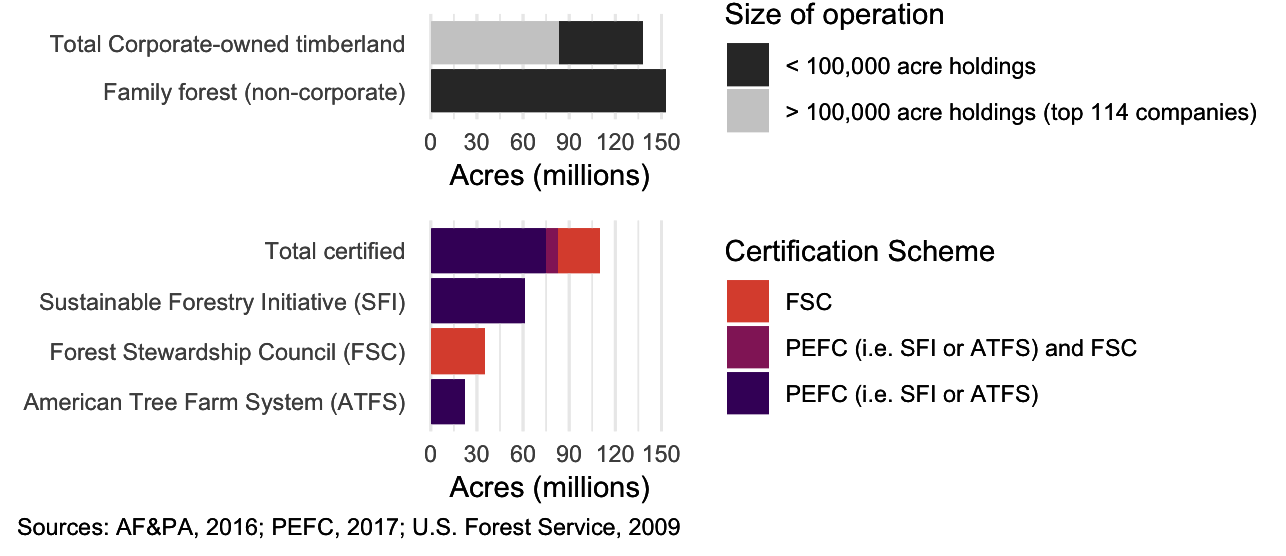
\includegraphics{acres-1.png}
\caption{U.S. Timberland by ownership and certification scheme}
\end{figure}

\emph{Origin of the FSC:} The FSC was established as an international
non-profit organization in 1993 by a group of environmental and social
advocacy organizations, academics, indigenous groups, and companies.
FSC's founders designed its rulemaking procedures as a ``democratic''
process where members vote on decision-making rules as well as
substantive policy \citep{Meidinger2003}. FSC standards begin with a set
of international ``Principles and Criteria'' (FSC--P\&C) that are used
by national-level organizations to develop more specific indicators. Our
analysis of the FSC in the U.S. thus assesses both the international
P\&C and the FSC-US national standard.

\emph{Origin of the SFI:} In 1995, in response to the emergence of the
FSC, the U.S.-based industry association, the American Forest \& Paper
Association, established a forest management standard and required its
members (most of the U.S. forest products industry) to support it.
Optional third-party auditing was added in 1998, which became mandatory
in 2002, the same year that the American Forest \& Paper Association
made the SFI a legally distinct entity with a rulemaking process that is
formally independent, though still largely governed by business
stakeholders. The SFI has since been endorsed by the global Program for
the Endorsement of Forest Certification (PEFC). The PEFC maintains a set
of Sustainable Forest Management Benchmarks intended to guide
participating programs, many of which are industry-backed alternatives
to the FSC. Unlike the FSC--P\&C, the PEFC does not require the SFI and
other national-level programs to adopt its benchmarks verbatim. Instead,
they are expected to demonstrate the ``equivalence'' of their standards
with PEFC benchmarks. This means that national standards like the SFI's
can have, by some measures, less stringent requirements than PEFC
benchmarks.

\emph{``Sustainable'' Forestry:} Like many sectors, there are ongoing
debates over acceptable business practices and the appropriate role of
public and private regulation in forestry. ``Sustainable'' forestry has
many meanings \citep{McDermott2012}. For example, some programs use
``natural'' conditions or functions as benchmarks for sustainability,
involving complex choices about what is ``natural'' and what degree of
naturalness is appropriate. In other conceptions, ``sustainable'' is
less associated with naturalistic management and more about the
long-term efficiency of production. Such differences manifest in
distinct goals and different means to achieve them. A regulation
targeting efficiency may require high levels of utilization of trees and
tree-parts, whereas a regulation targeting naturalistic management may
include requirements to leave economically valuable timber behind for
animal habitat or soil health. Disagreements become concrete in the
details of such requirements. Thus, a meaningful assessment of
similarities and differences between regulations requires attention to
detail.

\subsection{Scope, prescriptiveness, and policy settings in
forestry}\label{scope-prescriptiveness-and-policy-settings-in-forestry}

To measure comprehensiveness of scope, we reviewed all FSC, PEFC and SFI
standards in effect between 2008 and 2016 to assess their coverage
across 48 distinct ``key issues'' covering a broad scope of forestry
requirements, from employee wages and resource utilization to
protections for endangered species and indigenous peoples' rights. These
issues were selected in 2008 using an iterative process to disaggregate
forestry policies to capture all of the key issues addressed by FSC,
PEFC, and SFI requirements \citep{McDermott2010}.

To measure prescriptiveness, we assess the precise wording of the text
on each issue. If firms have discretion among performance levels, only
the least demanding levels are prescriptive. For example, if firms are
required to ``maintain or enhance'' water quality, the option to merely
``maintain'' means that there is no mandatory requirement to ``enhance''
water quality.

To measure policy settings, we offer detailed issue-by-issue comparisons
of performance requirements on most of our 48 key issues in the text
below and all of them in the online appendix. This approach is similar
to how previous scholars have descriptively compared the SFI and FSC
standards on select sets of issues, except with a comprehensive scope of
potential issues. Doing so allows us to classify each specific change,
the types of issues that changed, and difference on issues that may be
important but not (yet) salient in the public debates.

\subsection{Results}\label{results}

Here we compare each standard to its previous version and the
contemporary version from its competitor. We assess revisions in the
FSC- International's 2012 Revised Principles and Criteria 01-001 Version
5-0 (FSC--P\&C) and compare them to revisions in the PEFC's Sustainable
Forest Management Standards 1003:2010. Similarly, we compare the 2010
FSC-U.S. Forest Management Standard Version 1.0 to the FSC-US National
Indicators and regional standards it replaced and compare these to the
2005-2009, 2010--2014, and 2015-2019 SFI standards. Unless otherwise
specified, ``FSC-US'' and ``SFI'' refer to the version of each standard
in effect in 2016. We do not fully capture subnational variation. The
FSC-US standard recognizes nine different sub-national regions. Some
have additional indicators, meaning that, in some states, FSC standards
were more prescriptive or had higher performance thresholds than our
findings reflect (see the online appendix).

\subsubsection{Comparing FSC's and PEFC's international
requirements}\label{comparing-fscs-and-pefcs-international-requirements}

\emph{Scope:} The FSC-P\&C and PEFC maintained a similar scope of issues
covered (see the top panel of Figure 2). The PEFC once covered slightly
fewer issues than did the FSC-P\&C, but its 2010 revisions added new
requirements on eight key issues that it previously did not address,
making the two programs generally aligned in the scope of issues
covered. As of 2015, the FSC P\&C covered three potentially costly
issues that the PEFC still did not: carbon emissions, restrictions on
conversion to plantations, and worker wage requirements (see the middle
panel of Figure 2). PEFC covers two issues relating to public
perceptions that FSC-P\&C do not: managing the aesthetic impacts of
forestry and allowing public access.

\emph{Prescriptiveness:} Overall, the FSC maintained more prescriptive
requirements in its Principles \& Criteria than the PEFC benchmarks (the
top panel of Figure 2), but the PEFC moved closer to the FSC-P\&C in
some key areas (the middle panel of Figure 2). These include additional
requirements on issues including indigenous rights, community benefits,
and public reporting and consultation (see the online appendix for
specific language). The PEFC became at least as prescriptive as the
FSC--P\&C on over half of key issues. In absolute terms, the PEFC
increased prescriptiveness on 19 key issues and decreased on none,
whereas the FSC--P\&C increased on 13 and decreased on four. Yet
significant differences remain. The FSC-P\&C contain more prescriptive
language on most ecological criteria, including protected areas and
restrictions on conversion to plantations.

Both programs have more procedural requirements than substantive
requirements (i.e., they are more focused on process than outcomes).
Despite convergence in the PEFC's revised requirements, the FSC-P\&C
remained more prescriptive than PEFC requirements on 17 of the 48 key
issues whereas PEFC requirements are more prescriptive on nine issues,
with both programs being equally prescriptive on 19 issues. Because the
PEFC started at a lower level but increased prescriptiveness on more
issues than did FSC P\&C, the resulting pattern is an ``upward
convergence'' (the bottom panel of Figure 2).

\begin{figure}
\centering
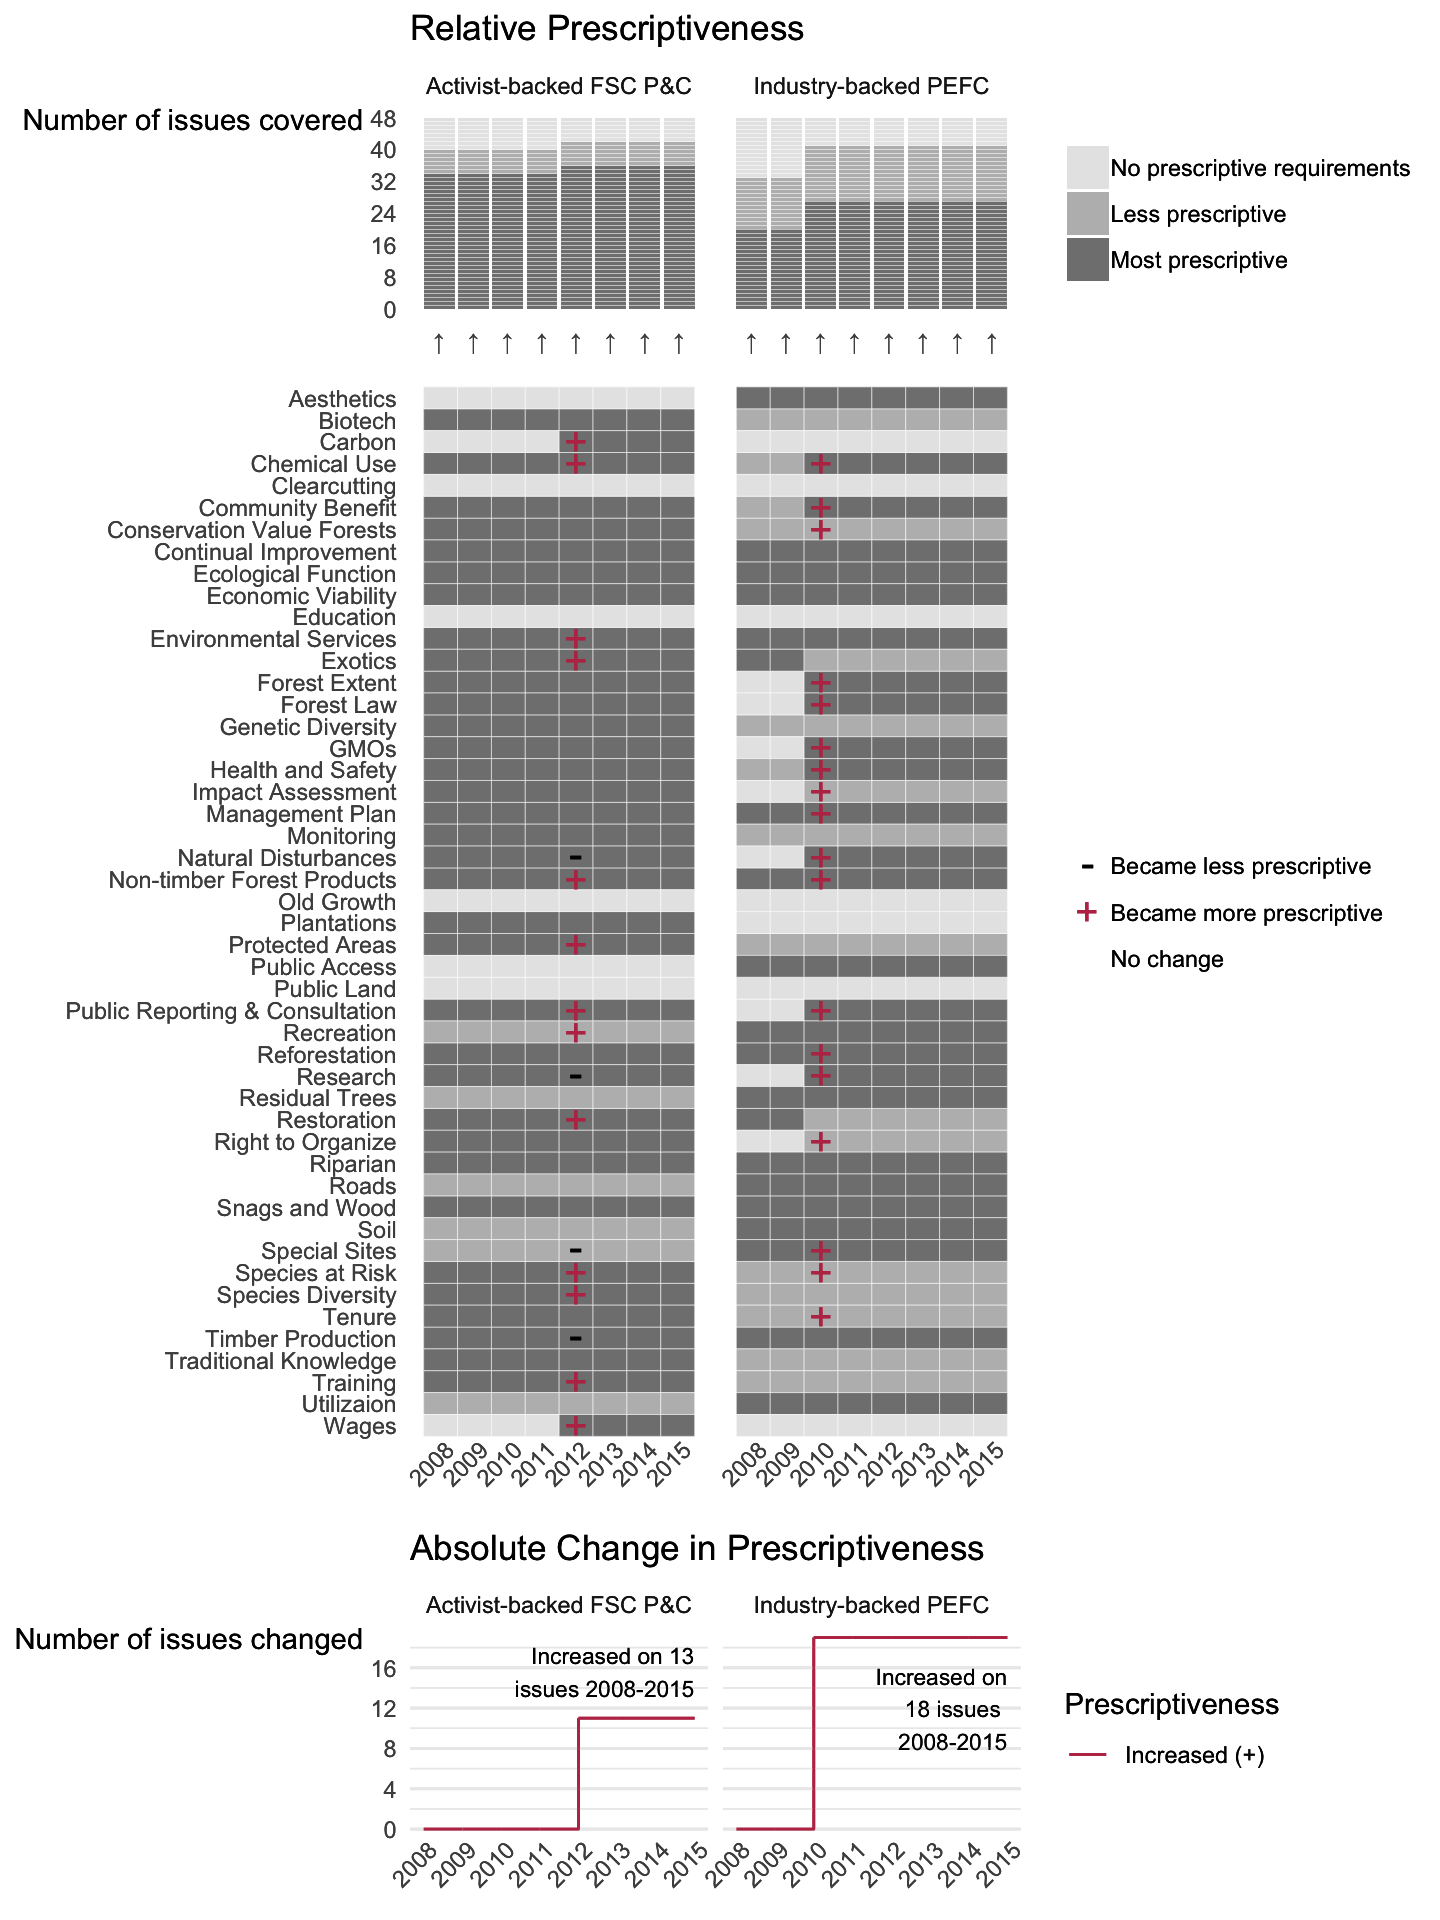
\includegraphics{FSC-PEFC-1.png}
\caption{Scope and Prescriptiveness of FSC P\&C and PEFC 2008-2015}
\end{figure}

\emph{Policy settings:} One particularly controversial issue is the
conversion of natural forests to timber plantations. Both programs
permit certification of natural forest converted to plantation forestry
under ``justifiable circumstances,'' which differ qualitatively between
the two programs. For the FSC, this means that conversion has ``clear,
substantial, additional, secure, long-term conservation benefits.'' For
the PEFC it means that conversion must have ``long-term conservation,
economic, and social benefits.'' They also differ regarding the extent
of forest conversion allowed. The FSC-P\&C allow companies to convert
``limited areas'' while the PEFC allows ``small proportions of forest
types.'' Both standards specify that conversion must not damage
culturally or socially significant areas, but whereas PEFC suggests that
forests should only be certified if the conversion occurred before 2011,
the FSC-P\&C require that conversion occurred before 1994, significantly
different thresholds.

Both FSC-P\&C and PEFC added new requirements on socio-economic issues,
land tenure rights, and stakeholder consultations. In addition to citing
the UN Declaration on Rights of Indigenous Peoples, both programs
included criteria that require free, prior and informed consent of
indigenous peoples and local communities. The FSC-P\&C required ``free
and informed consent'' concerning control over forest operations and
compensation for the use of traditional knowledge. Both standards also
recognized legal, traditional, and customary rights. However, the
FSC-P\&C are more prescriptive, defining topics on which forest managers
must consult with indigenous peoples, while the PEFC standards are more
procedural, requiring only that engagement takes place. The FSC's
criteria regarding public consultation include special obligations to
``affected stakeholders'' compared to ``interested stakeholders'' while
PEFC requirements regarding ``local people and other stakeholders'' are
the same.

Both programs cover similar ecological issues, with some qualitative
differences. Both FSC--P\&C and PEFC requirements prohibited the use of
GMOs in the area being certified, with some possible flexibility should
scientific evidence affirm the safety of GMO trees. FSC--P\&C allow
documented and monitored use of biological control methods but
prohibited a specific list of ``Highly Hazardous Chemicals.'' The PEFC
added prohibitions on pesticides that remain biologically active and
highly toxic pesticides where viable alternatives are available. The
PEFC explicitly required managers to avoid chemicals where they threaten
water quality, while FSC--P\&C water protection criteria were less
explicit. Both programs had similar requirements for sustainable
production of timber and non-timber forest products (NTFPs), but the
FSC-P\&C set a higher level of protection for animal habitat. While the
FSC--P\&C required protection of rare and threatened species and their
habitats, the PEFC only required that protected and endangered species
not be exploited for commercial purposes and that managers take measures
for their protection ``where necessary,'' without defining these
conditions.

\emph{Summary:} Overall, while the PEFC added more requirements
concerning indigenous rights and labor standards and came to cover a
similar scope of issues to the FSC P\&C, the FSC-P\&C remained more
prescriptive on social issues and significantly more prescriptive on
ecological issues. Compared to the prescriptiveness of the FSC-US and
SFI described below, the FSC--P\&C and PEFC requirements exhibited more
convergence on both scope and prescriptiveness (compare Figures 3 and 4)
though many differences in policy settings remained.

\subsubsection{Comparing the FSC-US and
SFI}\label{comparing-the-fsc-us-and-sfi}

\emph{Scope:} Consistent with the international level, the
activist-backed FSC-US program and industry-backed SFI program in the
United States address a similar scope of issues, but the FSC-US is more
prescriptive on most (the top panel of Figure 3). As of 2016, the FSC-US
did cover six potentially costly issues that the SFI did not; community
benefit requirements, forest extent restrictions, required impact
assessments, protected area restrictions, restoration requirements, and
indigenous tenure protections (the middle panel of Figure 3). The SFI,
in turn, covered one issue that the FSC-US did not: contributing to
forestry research. Both programs added requirements on greenhouse gasses
in 2010. SFI allows for the conversion of natural forests to plantations
if ecological impacts are not significant and the converted forest type
is not rare, but in 2015, SFI added a requirement to conduct an
assessment of these impacts. Yet, the FSC-US still maintained more
prescriptive requirements, only allowing certification of plantation
forests if they were converted from natural forests before 1994. FSC-US
also requires a portion of these plantations to be maintained as, or
restored to, natural conditions.

\emph{Prescriptiveness:} In 2008 the FSC-US was more prescriptive on 36
of 48 key issues, and the SFI was more prescriptive on five issues.
These five are some of the most ``business-friendly'' issues: continual
improvement of management planning, educating the public about forestry,
contributions to forestry research, worker training, and efficient
material utilization. In 2016 the FSC-US was more prescriptive on 37 key
issues, and the SFI was more prescriptive on the same five issues. The
two standards were equally prescriptive on five issues. This means that
the FSC-US had the ``most prescriptive'' requirements---those as
prescriptive or more than any other program---on 42 issues and the SFI
had the most prescriptive requirements on 10 (the top panel of Figure
3).

Counting changes made to the FSC-US and SFI standards between 2008 and
2016 reveals an ``upward diverging'' pattern, where the FSC-US became
more prescriptive than did the SFI (the bottom panel of Figure 3). Of 48
key issues, the FSC-US became more prescriptive on 20, whereas SFI
became more prescriptive on 12 (eight in 2010, one more in 2013, and
three more in 2015).

\begin{figure}
\centering
\includegraphics{FSC-SFI-1.png}
\caption{Scope and Prescriptiveness of FSC-US and SFI 2008-2016}
\end{figure}

\emph{Policy Settings:} Issues such as clearcut size limits and limits
on harvesting near streams clearly illustrate enduring differences
between the SFI and the FSC-US because we can compare policy settings on
these issues both qualitatively and quantitatively. Qualitatively, the
FSC-US increasingly restricts the size and shape of clearcuts to reflect
``natural disturbance'' and maintain ecological functions regardless of
how it looks, whereas the SFI emphasizes ``the visual impacts of
forestry'' and requires rapid site ``green-up.'' Quantitatively, the SFI
limited clearcuts for all forest types to an average of 120 acres with
no maximum and no limits for harvesting with 20 percent tree retention
(i.e., intensive but not clearcut harvesting). In contrast, the FSC-US
limits clearcuts to a 40-acre average and 80-acre maximum, with
additional restrictions based on region and forest type. The FSC-US also
limits harvesting with 20 percent tree retention to a 100-acre average
and 80-acre maximum, with further restrictions based on region and
forest type (Figure 4).

For harvesting near streams, the FSC-US lists specific requirements for
water quality, habitat, and other objectives with a focus on
restoration. Additionally, most FSC-US regions have numeric minimum
riparian buffer zones (Figure 5). In 2015, SFI expanded its definitions
of riparian areas but continued to allow more discretion regarding what
managers include in plans to protect water resources with no numerical
minimum buffers beyond those in state laws and best management
practices. While we can only compare most other policy settings
qualitatively, the FSC-US clearly requires higher levels of performance
on many social and ecological issues (Table \ref{issues}).

\begin{figure}
\centering
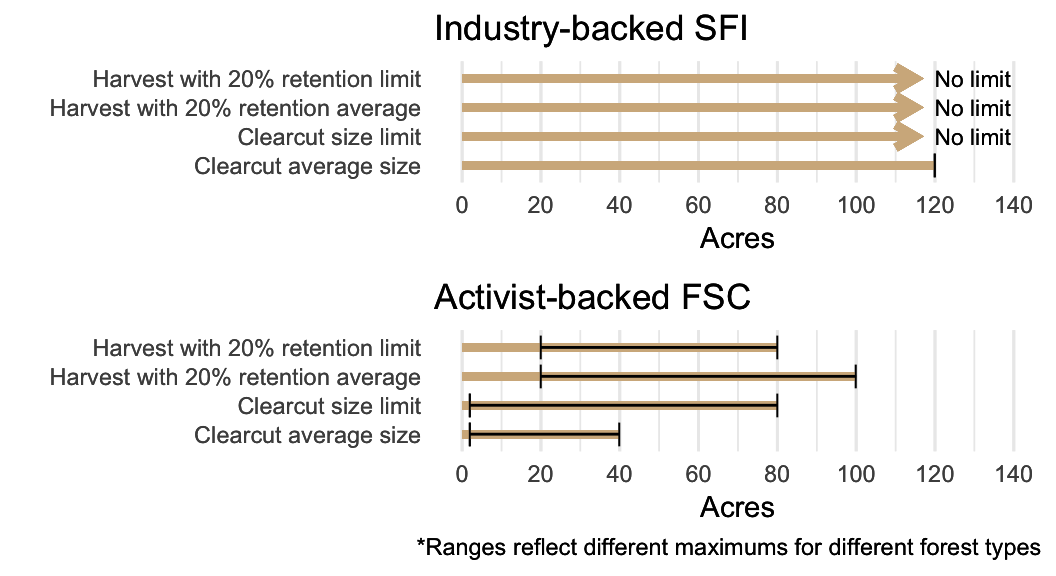
\includegraphics{clearcuts-1.png}
\caption{Limits on Clearcut Size\label{clearcuts}}
\end{figure}

\begin{figure}
\centering
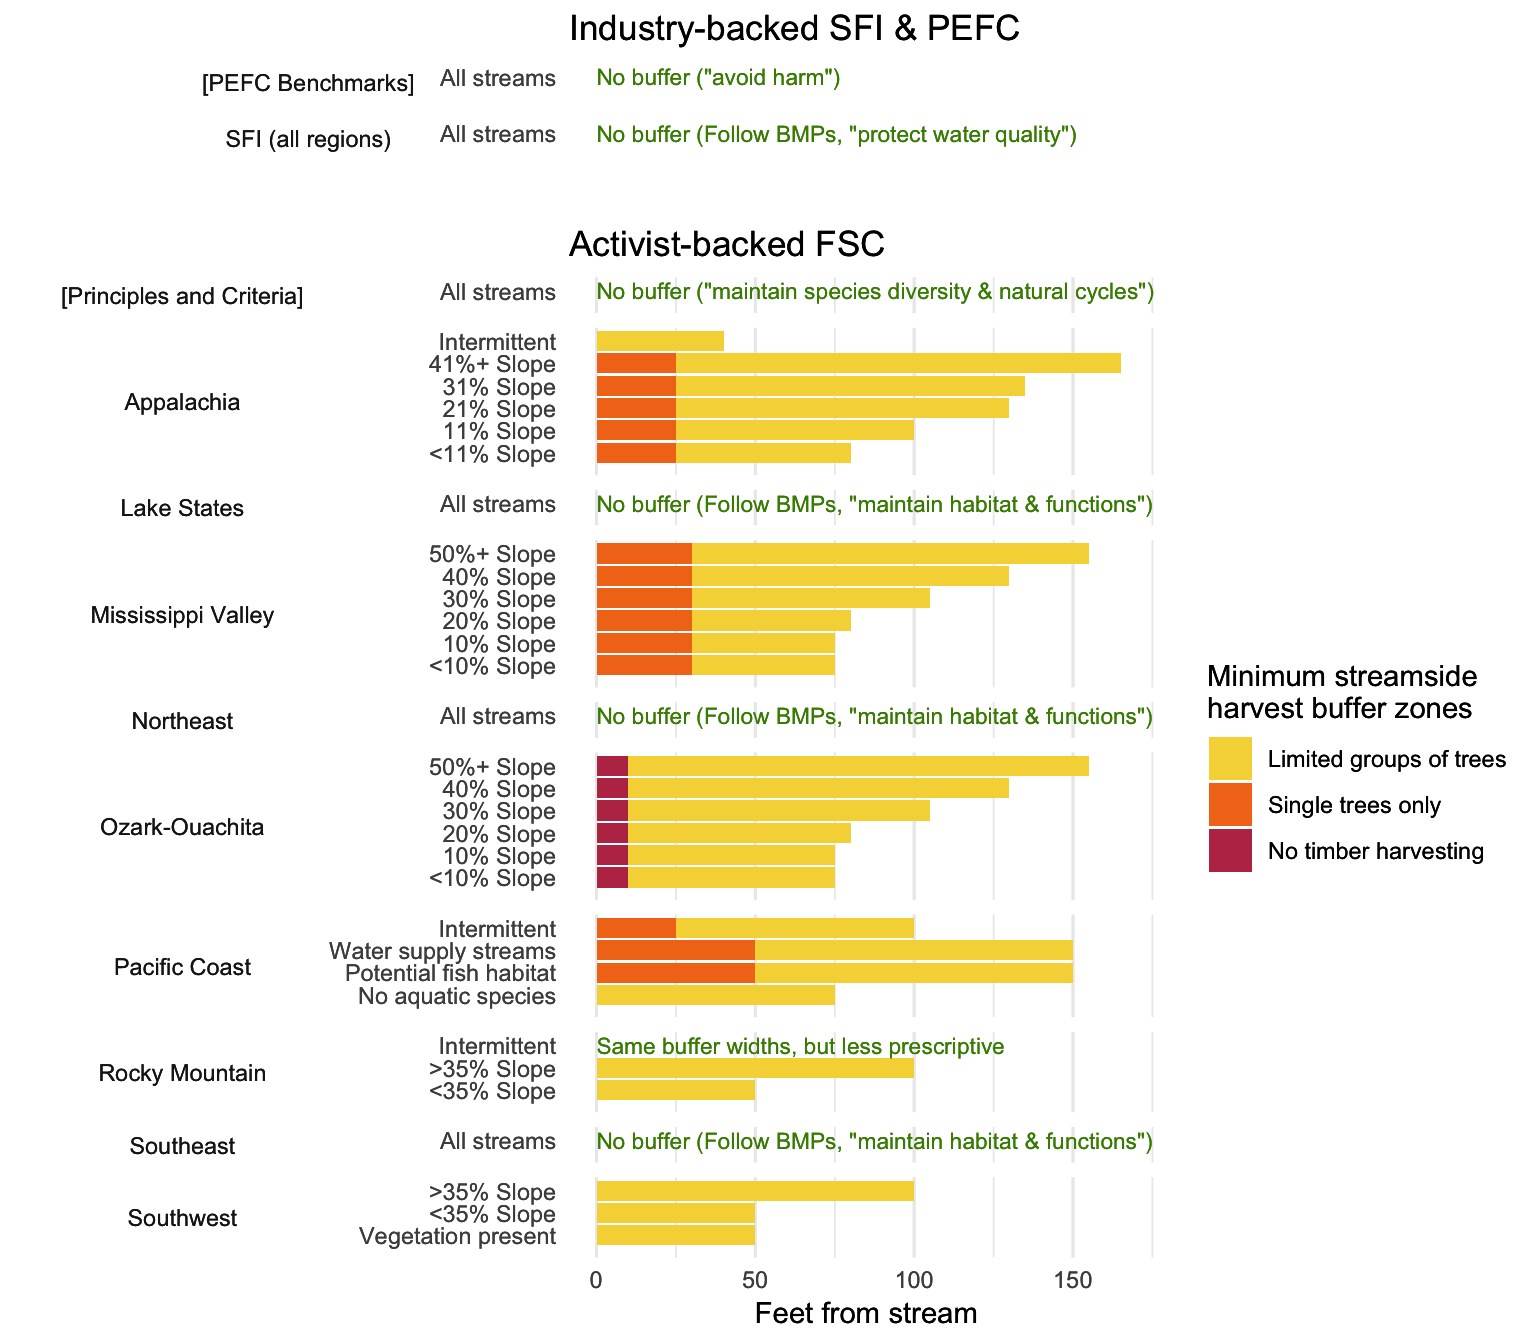
\includegraphics{riparian-1.png}
\caption{Limits on Harvesting Near Streams\label{riparian}}
\end{figure}

\begin{longtable}[]{@{}lll@{}}
\toprule
\begin{minipage}[b]{0.20\columnwidth}\raggedright\strut
Issue\strut
\end{minipage} & \begin{minipage}[b]{0.36\columnwidth}\raggedright\strut
Activist-backed FSC-US\strut
\end{minipage} & \begin{minipage}[b]{0.36\columnwidth}\raggedright\strut
Industry-backed SFI\strut
\end{minipage}\tabularnewline
\midrule
\endhead
\begin{minipage}[t]{0.20\columnwidth}\raggedright\strut
Indigenous peoples' rights\strut
\end{minipage} & \begin{minipage}[t]{0.36\columnwidth}\raggedright\strut
Recognize and uphold rights, customs, culture including UNDRIP. No
threat to rights or resources. Free, prior, and informed consent on
public and private lands. Engage indigenous peoples and consult with
affected groups. Cooperate to identify and protect significant sites.
Compensate for indigenous knowledge and utilize as requested.\strut
\end{minipage} & \begin{minipage}[t]{0.36\columnwidth}\raggedright\strut
A written policy acknowledging a commitment to recognize and respect
rights.\strut
\end{minipage}\tabularnewline
\begin{minipage}[t]{0.20\columnwidth}\raggedright\strut
Public Reporting and Consultation\strut
\end{minipage} & \begin{minipage}[t]{0.36\columnwidth}\raggedright\strut
Required on public and private lands.\strut
\end{minipage} & \begin{minipage}[t]{0.36\columnwidth}\raggedright\strut
Required on public lands.\strut
\end{minipage}\tabularnewline
\begin{minipage}[t]{0.20\columnwidth}\raggedright\strut
Forest conversion to non-forest\strut
\end{minipage} & \begin{minipage}[t]{0.36\columnwidth}\raggedright\strut
Prohibited except limited areas where clear, substantial, additional,
secure, long-term conservation benefits.\strut
\end{minipage} & \begin{minipage}[t]{0.36\columnwidth}\raggedright\strut
No specific policy.\strut
\end{minipage}\tabularnewline
\begin{minipage}[t]{0.20\columnwidth}\raggedright\strut
Old growth forest\strut
\end{minipage} & \begin{minipage}[t]{0.36\columnwidth}\raggedright\strut
Old growth is normally mapped as conservation forest. Only restoration
management on public land. Legacy trees not harvested. Maintain
structure, composition, and processes. A portion of the forest is
restored where old growth would naturally occur.\strut
\end{minipage} & \begin{minipage}[t]{0.36\columnwidth}\raggedright\strut
Support and participate in programs for old growth conservation in the
region --- no identification or restoration requirements.\strut
\end{minipage}\tabularnewline
\begin{minipage}[t]{0.20\columnwidth}\raggedright\strut
Protected areas\strut
\end{minipage} & \begin{minipage}[t]{0.36\columnwidth}\raggedright\strut
Conserve or restore a representative area of natural ecosystems. Assess
and maintain environmental values and necessary conservation
measures.\strut
\end{minipage} & \begin{minipage}[t]{0.36\columnwidth}\raggedright\strut
No specific policy.\strut
\end{minipage}\tabularnewline
\begin{minipage}[t]{0.20\columnwidth}\raggedright\strut
Threatened and Endangered Species\strut
\end{minipage} & \begin{minipage}[t]{0.36\columnwidth}\raggedright\strut
Survey and report or assume the presence of vulnerable, imperiled, and
critically imperiled. Maintain habitat \& viable populations.\strut
\end{minipage} & \begin{minipage}[t]{0.36\columnwidth}\raggedright\strut
Program to protect threatened and endangered species and known sites.
Protect viable occurrences of critically imperiled or imperiled
species.\strut
\end{minipage}\tabularnewline
\bottomrule
\end{longtable}

\textbar{}Threatened and Endangered Species \textbar{} Gap analysis,
identify and establish representative sample areas, survey for listed,
candidate, G1-G3, S1-S3, and N1-N3 designated species or assume
presence, report findings. Permanent protection of representative sample
of all habitats, conservation zones support viable populations.
\textbar{} Program to locate G1-G2 species through credible system, use
NatureServe or equivalent. Protect or manage special sites and sites
with special conservation value including vernal pools of ecological
significance, and sites with species at risk. \textbar{}

\textbar{}Indigenous use rights \textbar{} Access and use rights
documented, identified on maps \textbar{} Identify and protect
culturally important sites. \textbar{} \textbar{}Indigenous consultation
\textbar{} Identify and contact American Indian groups via designated
tribal representatives for legal or customary use rights, ensure no
impact on rights, protocols jointly developed and signed by tribes in
formal consultation, informed written consent, identify special sites
and protected areas. \textbar{} Confer with affected indigenous peoples
on public lands. \textbar{}Indigenous knowledge \textbar{} Understand
and respect traditional knowledge. \textbar{} Identify knowledge used,
fairly compensate for use. \textbar{} \textbar{}Workers' right to
organize \textbar{} Freedom to associate and advocate \textbar{} Develop
dispute resolution. \textbar{} Obey law. Train on worker rights.
\textbar{} \textbar{}Wages \textbar{} Meets local norms \textbar{}
Written commitment to comply with social law prevailing wage. Train on
wage rules. \textbar{} \textbar{}Safety \textbar{} posted safety
guidelines, contracts include safety, records kept \textbar{} Written
commitment to comply with OSHA. Training on OSHA \textbar{}



While both the FSC-US and SFI became more prescriptive, they did so to
different degrees and in different areas. The SFI's changes in 2010
emphasized issues related to industrial capacity (e.g., worker training
requirements) and reputation (e.g., managing the visual impact of
harvesting, communicating with stakeholders about logging, and educating
the public about forestry), issues where SFI already had the most
prescriptive requirements. Changes made the same year by the FSC-US
emphasized conservation-oriented forestry while removing a training
requirement.

The bulk of the divergence occurred on ecological requirements like
protecting habitat, where the FSC-US became more prescriptive while the
SFI stayed constant or, in the case of preserving old-growth forests,
decreased in prescriptiveness. Regarding protected areas, the FSC-US
continued to require that managers preserve representative samples of
habitats, but, since 2010, also requires an assessment of the adequacy
of permanent protections. SFI's requirements for protected areas
continue to be encompassed mainly by its requirements to protect
imperiled species. SFI continues to require plans to identify and
protect moderately to highly valuable known populations of imperiled or
critically imperiled species (designations G1-G2). In contrast, the
FSC-US expanded the scope of species requiring protection in 2010 to
include natural heritage species and candidate species (designations
G1-G3, S1-S3, N1-N3). The FSC-US added requirements to conduct surveys
for any at-risk species potentially present or presume that listed or
candidate species are present if the forest is in a species' range. For
old-growth forests, in 2010, the FSC-US added prescriptive requirements
to restore a portion of old-growth forests where they would naturally
occur, and it continues to demand protection measures that prohibit
harvesting in most cases. In 2010, SFI removed a requirement to maintain
sufficient old-growth acreage to maintain biodiversity, but in 2015
added a requirement to participate in conservation planning.

The FSC-US and SFI's changing requirements to designate and protect
conservation areas exemplify their overall upwardly diverging
prescriptiveness, with the SFI adding some prescriptive requirements but
the FSC-US adding even more prescriptive requirements. In 2010, the SFI
added new requirements to collect data on ``Forests of Exceptional
Conservation Value'' (FECV), which we compare to the FSC's requirements
for ``High Conservation Value Forests'' (HCVF). Also, in 2010, the
FSC-US added language regarding monitoring and adaptive management of
HCVFs. While the acronyms and even the additional language appear
similar, the SFI allowed more flexibility in FECV management. HCVFs
under the FSC-US required significantly more than baseline practices
\citep{Newsom2005}, while SFI's FECV requirements have been criticized
as not significantly exceeding legal baselines (state and federal
endangered species acts) which already protect threatened and endangered
species. The FSC-US then added even more prescriptive requirements
requiring certain areas to be designated HCVFs and prescriptive
accountability mechanisms for HCVF management.

\emph{Summary:} Overall, each program had distinct areas in which its
requirements were more prescriptive. For the FSC, these requirements
tended to demand that forest operations ``resemble natural processes''
and ``maintain ecosystem function.'' This language appeared more
frequently and forcefully in the 2010 standard concerning issues
including clearcutting, riparian management, HCVFs, protected areas,
old-growth forests, snags and downed wood, residual trees, genetic
diversity, plantations, restoration, natural disturbance, non-timber
forest products, soil protection, road building, and management
planning. In contrast, the SFI was most prescriptive on issues such as
material utilization, research, training, education, and public
reporting and consultation. The eight key issues on which the SFI
increased prescriptiveness in 2010 also reflect the SFI's focus on
industry capacity and reputation. These included aesthetics, public
reporting, education, training, and utilization.

The 2015 changes to the SFI standard reflect a different tack. In
contrast to the previous focus on more ``business-friendly'' issues
related to industry capacity and reputation, the three issues on which
the SFI increased prescriptiveness in 2015 reflect social and ecological
goals. These include prohibiting the use of certain toxic chemicals,
restricting the circumstances under which natural forests can be
converted to plantations, and requiring a written policy to recognize
and respect indigenous rights.

\section{Discussion}\label{discussion}

\subsection{Overall comparison}\label{overall-comparison}

By distinguishing different types of stringency on a comprehensive set
of issues, our framework improves upon blunt measures of ``high'' or
``low'' standards based on generalizations or on only a few issues.

Overall our results are consistent with the expectation that activist
backed programs have higher levels of more costly types of stringency.
On ecological goals, the FSC-US standard was significantly more
stringent than the SFI standard on both scope and prescriptiveness
dimensions. On social goals, results are more mixed. On scope, the
FSC-US standard protected land tenure and requires that local
communities benefit from harvesting in ways that were unmatched by SFI's
standard. Numerically, FSC-US had a broader scope of social benefits,
but the programs did present tradeoffs between conceptions of the public
good. On prescriptiveness, the contrast was more stark, with the FSC-US
standard having significantly more prescriptive requirements on most
social issues. On policy settings, the two programs had significant
differences. On labor standards and indigenous rights, the FSC-US
required higher wages and more attention to rights than did the SFI. In
short, by conventional definitions of what counts as a social issue, by
most qualitative comparisons, and certainly in terms of
prescriptiveness, the FSC-US standard was more stringent than the SFI
standard on social issues.

On more business-oriented goals such as efficiency (e.g.~levels of cut
tree utilization), industry capacity (e.g.~workforce training and
research), and industry reputation (e.g., public education and
aesthetics), the patterns were largely reversed. SFI was slightly
broader in scope, requiring contributions to research where FSC did not,
was more prescriptive, and required increasingly demanding performance
levels on many business-friendly issues.

\subsection{Patterns of change}\label{patterns-of-change}

In most years between 2008 and 2016, neither the FSC nor the SFI changed
on any issue (the center cell in Table \ref{patterns}, ``equilibrium'').

When they did change, upwardly diverging prescriptiveness was the
dominant pattern. Most changes for both programs occurred in 2010 where
the overall pattern was divergence, rather than convergence or
stability. For all sixteen issues on which only the FSC-US added
requirements, it already had the more prescriptive requirements, and
almost all of these additions address ecological problems. Similarly,
for three out of the four issues on which only the SFI added
requirements, the SFI already had more prescriptive requirements.

The vast majority of changes (twenty-one of twenty-seven issues changed)
fit a pattern where one program increased prescriptiveness while the
other did not (or in one case, increased to a lesser degree) and the
program that increased stringency already had the more prescriptive
requirements. On eighteen issues, the less prescriptive program stayed
the same, leading to upward divergence. On three issues, the less
prescriptive program decreased prescriptiveness, leading to opposing
divergence (see Table \ref{patterns-2010-2015}).

\begin{table}
\caption{2010 and 2015 Patterns of Change in Prescriptiveness among U.S. Forestry Certification Programs (FSC-US and SFI) on 48 Key Issues}
\label{patterns-2010-2015}
\raggedright

2010

\begin{longtable}[]{@{}lccc@{}}
\toprule
& Converging & Parallell & Diverging\tabularnewline
\midrule
\endhead
Increasing & 1 & 3 & 18\tabularnewline
Opposing or Eqilibrium & 0 & 21 & 3\tabularnewline
Decreasing & 2 & 0 & 0\tabularnewline
\bottomrule
\end{longtable}

2015

\begin{longtable}[]{@{}lccc@{}}
\toprule
& Converging & Parallell & Diverging\tabularnewline
\midrule
\endhead
Increasing & 3 & 0 & 0\tabularnewline
Opposing or Eqilibrium & 0 & 45 & 0\tabularnewline
Decreasing & 0 & 0 & 0\tabularnewline
\bottomrule
\end{longtable}

\end{table}

Convergence was rare. In 2010, upward convergence only occurred where
FSC-US added requirements on the issue of ``continual improvement'' of
harvesting operations, an issue usually associated more with the SFI.
This outcome is interesting because scholars generally predict that less
stringent private regulations will converge toward ``benchmark''
standards like FSC's \citep{Overdevest2005, Overdevest2010}. Instead, we
find the FSC-US ratcheting up prescriptiveness on an issue where its
industry-backed competitor had more stringent requirements. Indeed, most
studies overlook the possibility that industry-backed standards like the
SFI may be more stringent on some issues and thus fail to theorize about
dynamics that could cause this. We see downward convergence only on the
issues of ``community benefits'' and ``tenure rights,'' where the more
prescriptive FSC-US removed requirements, thus moving closer to SFI.

Parallel change was also rare. An upward parallel change occurred on
only three issues in 2010: forest management planning, controlling
carbon emissions, and reporting and consultation, where both programs
added requirements. We classify the addition of protections for riparian
zones by both SFI and FSC-US as another case of upward divergence rather
than upward parallel change because the requirements for riparian
protection added by the FSC-US were more prescriptive than those added
by the SFI. No issues exhibited downward parallel change, as ``race to
the bottom'' theory anticipates.

After the significant revisions of both programs in 2010, only the SFI
updated its requirements, mostly in 2015. In contrast to the 2010
changes, the pattern in 2015 was a moderate upward convergence. SFI
increased prescriptiveness on three issues where it did not already have
the most prescriptive requirements. While a much smaller scale of change
than 2010, this upward convergence is notable because it focuses on
regulating toxic chemicals, plantations, and harvesting on tribal lands,
which likely have net costs rather than benefits for the industry.

\subsection{Implications for theory}\label{implications-for-theory}

Applying our framework to the case of forestry certification reveals how
one could reach different conclusions by looking at different dimensions
of change. If focusing only on program scope, one would find little
support for any theory predicting change---either convergence or
divergence. If focusing only on prescriptiveness on ecological issues,
one would find divergence, with the activist-backed FSC-US becoming more
prescriptive at a faster rate than the industry-backed SFI. But if
focusing only on prescriptiveness on industry capacity and reputation
issues, one would find the opposite, with the SFI becoming more
prescriptive at a faster rate than the FSC-US. While certainly
inconsistent with ``race-to-the-bottom'' theories, the overall upward by
diverging trajectories of the SFI and FSC-US do not exactly fit a ``race
to the top'' either.

Our results do support, with some caveats, hypotheses 1.1, 2.1 , and 2.2
outlined in Section 2.3. We ended up with no evidence either way on
hypothesis 1.2.

Regarding H1.1, the industry-backed program often had language similar
to that of the activist-driven standard (i.e., it had a similar scope),
but often lacked mandatory performance thresholds (i.e., it did not have
similar prescriptiveness). If ``talk is cheap,'' but prescriptive
requirements are costly, it makes sense that an industry-backed program
would cover similar issues as its competitor without adopting costly
performance thresholds. This result suggests that any test of theories
about the cost of compliance must distinguish between measures of
stringency based on policy scope or prescriptiveness. Regarding H1.2, we
cannot tell whether changes in scope are more likely to be matched by
competing programs because neither program changed significantly in the
scope of issues addressed. Both programs did begin regulating carbon
emissions in 2010, but it is unclear if this change in scope is one
program reacting to the other or both programs responding to a third
causal factor.

Regarding H2.1, we find differentiation between the FSC-US and the SFI;
the activist-backed program was more comprehensive in scope, was more
prescriptive, and had higher performance levels on issues that cost
firms', while the industry-backed program was more comprehensive in
scope, was more prescriptive, and had higher performance levels on
issues that create net utility for the industry. Hypothesis 2.2 posits
that the same kind of differentiation will drive policy change. This
aligns with changes to the FSC-US and SFI in 2010, but less so in 2015.
More research is needed to test these and other hypotheses, using
similarly precise and comprehensive measures of regulatory stringency.
Specifically, while ``ratcheting up'' theories anticipate the general
upward direction we observe, more attention is needed to explain why
programs may increase prescriptiveness on different issues, especially
issues where they already have the more stringent requirements.

\subsection{Industry-backed certification programs as a form of
collective
action}\label{industry-backed-certification-programs-as-a-form-of-collective-action}

Our finding that the SFI and FSC-US were each more prescriptive and
continued to become more prescriptive on qualitatively different issues
highlights how industry-backed certification programs can serve their
industry in two ways. First, they provide individual firms with a
service---a signal of ``social responsibility'' that requires a credible
third party. Such a signal would be more expensive to send by complying
with an activist-backed regulation. Second, they provide a mechanism for
an industry to improve its collective reputation and capacity by
coordinating contributions to collective goods, a common function of
industry associations.

Regarding the first, industry-backed programs are often created to save
firms money by offering a label that sends ``green'' or ``socially
responsible'' signals in the market without some of the more costly
demands of activist-backed programs or public regulations. Such signals
are often based on perceived stringency, which may vary from actual
stringency. \footnote{While our framework clarifies differences in
  actual stringency between activist- and industry- backed programs,
  which program one prefers will still depend on one's problem
  definitions and values. What we do know is that, on many issues,
  industry-backed programs address the same issues as activist-backed
  programs with language that might give the impression of equivalence
  in stringency but contain substantially fewer prescriptive
  requirements. We show that seemingly similar looking language requires
  very different levels of performance. For example, the SFI
  requirements for ``Forests of Exceptional Conservation Value'' (FECV)
  are much less prescriptive than the FSC-US requirements for ``High
  Conservation Value Forests'' (HCVF), despite their similar language
  (also see (e.g.~Figures \ref{riparian} and \ref{clearcuts} and Table
  \ref{issues}). The extent to which this helps firms coordinate to
  maximize the impression of stringency while minimizing the costs of
  doing so is a question for future research.} Nevertheless, maintaining
legitimacy may require some prescriptive requirements on costly issues.
On these issues levels of prescriptiveness and policy change are likely
driven by competition with activist-backed standards.

Regarding the second, the fact that the SFI developed more prescriptive
standards than the FSC-US on several issues is inconsistent with the
predictions that competition between industry-backed and activist-backed
competition will lead to a ``race to the bottom'' on all issues. It is
also inconsistent with the prediction that activist-backed standards
will be more prescriptive on all issues. However, the substance of these
issues suggests that these requirements are unrelated to competition
with the FSC. Instead, SFI had the most prescriptive requirements for
actions that firms may take anyway---like training workers and
maximizing efficiency---or that may be driven by their own collective
action problems---like managing the visual impact of harvesting and
sector-level reputation. Likewise, the three issues on which only the
SFI changed---maximizing the utilization of cut trees, public education,
and worker training---reflect concerns for the efficiency, reputation,
and capacity of the forest products industry. Educating the public about
forestry and training workers may not exclusively benefit individual
firms, but given the broad adoption of SFI certification, such
requirements may provide collective benefits for the sector in the form
of a positive public image and skilled workforce.

In short, where the SFI developed more prescriptive requirements than
the FSC, it required things that firms may do anyway (e.g., train
workers or educate the public), but have additional collective benefits
the more widely they are adopted. While unforeseen by existing theories,
the fact that the SFI is more prescriptive on some issues is
unsurprising if these requirements provide net benefits to the sector
regardless of activist pressures or consumer demands.

\section{Conclusion}\label{conclusion}

Scholars have made substantial progress in developing theories of how
economic and political forces shape the substance of private
regulations, and how these different requirements then affect levels of
adoption and compliance. We have argued that testing these theories
requires more precise statements of the types of policy substance to
which they apply and research that measures change across programs and
over time. Our framework for measuring regulatory stringency, and for
using longitudinal data to classify patterns of change, offers a
foundation for further research about how competing regulatory programs
compare, how they evolve, and why. There is no perfect way to compare
incommensurate policies. We have nonetheless made our best effort to
offer a method to do so. By applying this method, we have systematically
quantified differences that can be quantified and described as richly as
possible those comparisons that one can only make qualitatively.

Through the case of forestry standards in the U.S., we show what can be
gained by careful measurement of regulatory stringency and policy change
across a comprehensive scope of issues in a specific domain. Our results
show different patterns depending on whether one looks at policy scope,
prescriptiveness, or specific policy settings. Careful measurement
uncovered trends that previous scholarship has missed and which
contradict the predictions of several dominant theories. It also reveals
that apparent empirical debates in the literature are the result of
research design choices. Some scholars chose a few key issues and found
convergence. Others looked broadly and did not see it. We have looked
both precisely and broadly and found both conclusions were correct but
incomplete. Activist-backed and industry-backed programs converged in
policy scope on a few issues, but overall, their scopes have seen little
change. Furthermore, we found these programs to have diverged overall on
prescriptiveness, because, while both standards ``ratcheted up,'' they
did so at different rates and on different policy issues. We hope that
this deep dive into defining regulatory stringency and policy change in
one domain not only enables scholarship on the causes of public and
private regulation in forestry but that it also offers a model for
similar research in other policy domains.

This approach also has practical value. First, the power dynamics among
groups that promote programs like the FSC or the SFI have created an
environment in which competing claims about what exactly each program
requires and how this has changed confuse buyers. The politics of
private regulation revolve around ``public comparisons that would
resolve the debate about whose standards were higher''
\citep{Overdevest2010}. We offer concepts to clarify what ``higher''
standards may mean. Second, it is impossible to measure the impact of a
set of regulatory requirements without disentangling their component
parts. Thus, our analysis of written requirements is a necessary first
step for efforts to assess the effects on the ground.

Most importantly, our framework and analysis offer a model for careful
measurement of policy change as a variable. It is tempting to take
shortcuts by making broad generalizations or by selecting what is easy
to measure or what others have highlighted. However, if we aim to build
testable theories or collect the kinds of evidence needed to test
existing theories, our study illustrates the benefits of defining policy
change in ways that can be applied across programs and over time. Doing
so will not only improve the quality of research and theory, it may also
uncover entirely new puzzles and insights.
% --- PAGE: endnotes -----------------------
  \newpage 
  \theendnotes
% --- PAGE: refs -----------------------
\newpage
\singlespacing 
          \bibliography{certification.bib} 
  \end{document}
